
% Default to the notebook output style

    


% Inherit from the specified cell style.




    
\documentclass[11pt]{article}

    
    
    \usepackage[T1]{fontenc}
    % Nicer default font (+ math font) than Computer Modern for most use cases
    \usepackage{mathpazo}

    % Basic figure setup, for now with no caption control since it's done
    % automatically by Pandoc (which extracts ![](path) syntax from Markdown).
    \usepackage{graphicx}
    % We will generate all images so they have a width \maxwidth. This means
    % that they will get their normal width if they fit onto the page, but
    % are scaled down if they would overflow the margins.
    \makeatletter
    \def\maxwidth{\ifdim\Gin@nat@width>\linewidth\linewidth
    \else\Gin@nat@width\fi}
    \makeatother
    \let\Oldincludegraphics\includegraphics
    % Set max figure width to be 80% of text width, for now hardcoded.
    \renewcommand{\includegraphics}[1]{\Oldincludegraphics[width=.8\maxwidth]{#1}}
    % Ensure that by default, figures have no caption (until we provide a
    % proper Figure object with a Caption API and a way to capture that
    % in the conversion process - todo).
    \usepackage{caption}
    \DeclareCaptionLabelFormat{nolabel}{}
    \captionsetup{labelformat=nolabel}

    \usepackage{adjustbox} % Used to constrain images to a maximum size 
    \usepackage{xcolor} % Allow colors to be defined
    \usepackage{enumerate} % Needed for markdown enumerations to work
    \usepackage{geometry} % Used to adjust the document margins
    \usepackage{amsmath} % Equations
    \usepackage{amssymb} % Equations
    \usepackage{textcomp} % defines textquotesingle
    % Hack from http://tex.stackexchange.com/a/47451/13684:
    \AtBeginDocument{%
        \def\PYZsq{\textquotesingle}% Upright quotes in Pygmentized code
    }
    \usepackage{upquote} % Upright quotes for verbatim code
    \usepackage{eurosym} % defines \euro
    \usepackage[mathletters]{ucs} % Extended unicode (utf-8) support
    \usepackage[utf8x]{inputenc} % Allow utf-8 characters in the tex document
    \usepackage{fancyvrb} % verbatim replacement that allows latex
    \usepackage{grffile} % extends the file name processing of package graphics 
                         % to support a larger range 
    % The hyperref package gives us a pdf with properly built
    % internal navigation ('pdf bookmarks' for the table of contents,
    % internal cross-reference links, web links for URLs, etc.)
    \usepackage{hyperref}
    \usepackage{longtable} % longtable support required by pandoc >1.10
    \usepackage{booktabs}  % table support for pandoc > 1.12.2
    \usepackage[inline]{enumitem} % IRkernel/repr support (it uses the enumerate* environment)
    \usepackage[normalem]{ulem} % ulem is needed to support strikethroughs (\sout)
                                % normalem makes italics be italics, not underlines
    

    
    
    % Colors for the hyperref package
    \definecolor{urlcolor}{rgb}{0,.145,.698}
    \definecolor{linkcolor}{rgb}{.71,0.21,0.01}
    \definecolor{citecolor}{rgb}{.12,.54,.11}

    % ANSI colors
    \definecolor{ansi-black}{HTML}{3E424D}
    \definecolor{ansi-black-intense}{HTML}{282C36}
    \definecolor{ansi-red}{HTML}{E75C58}
    \definecolor{ansi-red-intense}{HTML}{B22B31}
    \definecolor{ansi-green}{HTML}{00A250}
    \definecolor{ansi-green-intense}{HTML}{007427}
    \definecolor{ansi-yellow}{HTML}{DDB62B}
    \definecolor{ansi-yellow-intense}{HTML}{B27D12}
    \definecolor{ansi-blue}{HTML}{208FFB}
    \definecolor{ansi-blue-intense}{HTML}{0065CA}
    \definecolor{ansi-magenta}{HTML}{D160C4}
    \definecolor{ansi-magenta-intense}{HTML}{A03196}
    \definecolor{ansi-cyan}{HTML}{60C6C8}
    \definecolor{ansi-cyan-intense}{HTML}{258F8F}
    \definecolor{ansi-white}{HTML}{C5C1B4}
    \definecolor{ansi-white-intense}{HTML}{A1A6B2}

    % commands and environments needed by pandoc snippets
    % extracted from the output of `pandoc -s`
    \providecommand{\tightlist}{%
      \setlength{\itemsep}{0pt}\setlength{\parskip}{0pt}}
    \DefineVerbatimEnvironment{Highlighting}{Verbatim}{commandchars=\\\{\}}
    % Add ',fontsize=\small' for more characters per line
    \newenvironment{Shaded}{}{}
    \newcommand{\KeywordTok}[1]{\textcolor[rgb]{0.00,0.44,0.13}{\textbf{{#1}}}}
    \newcommand{\DataTypeTok}[1]{\textcolor[rgb]{0.56,0.13,0.00}{{#1}}}
    \newcommand{\DecValTok}[1]{\textcolor[rgb]{0.25,0.63,0.44}{{#1}}}
    \newcommand{\BaseNTok}[1]{\textcolor[rgb]{0.25,0.63,0.44}{{#1}}}
    \newcommand{\FloatTok}[1]{\textcolor[rgb]{0.25,0.63,0.44}{{#1}}}
    \newcommand{\CharTok}[1]{\textcolor[rgb]{0.25,0.44,0.63}{{#1}}}
    \newcommand{\StringTok}[1]{\textcolor[rgb]{0.25,0.44,0.63}{{#1}}}
    \newcommand{\CommentTok}[1]{\textcolor[rgb]{0.38,0.63,0.69}{\textit{{#1}}}}
    \newcommand{\OtherTok}[1]{\textcolor[rgb]{0.00,0.44,0.13}{{#1}}}
    \newcommand{\AlertTok}[1]{\textcolor[rgb]{1.00,0.00,0.00}{\textbf{{#1}}}}
    \newcommand{\FunctionTok}[1]{\textcolor[rgb]{0.02,0.16,0.49}{{#1}}}
    \newcommand{\RegionMarkerTok}[1]{{#1}}
    \newcommand{\ErrorTok}[1]{\textcolor[rgb]{1.00,0.00,0.00}{\textbf{{#1}}}}
    \newcommand{\NormalTok}[1]{{#1}}
    
    % Additional commands for more recent versions of Pandoc
    \newcommand{\ConstantTok}[1]{\textcolor[rgb]{0.53,0.00,0.00}{{#1}}}
    \newcommand{\SpecialCharTok}[1]{\textcolor[rgb]{0.25,0.44,0.63}{{#1}}}
    \newcommand{\VerbatimStringTok}[1]{\textcolor[rgb]{0.25,0.44,0.63}{{#1}}}
    \newcommand{\SpecialStringTok}[1]{\textcolor[rgb]{0.73,0.40,0.53}{{#1}}}
    \newcommand{\ImportTok}[1]{{#1}}
    \newcommand{\DocumentationTok}[1]{\textcolor[rgb]{0.73,0.13,0.13}{\textit{{#1}}}}
    \newcommand{\AnnotationTok}[1]{\textcolor[rgb]{0.38,0.63,0.69}{\textbf{\textit{{#1}}}}}
    \newcommand{\CommentVarTok}[1]{\textcolor[rgb]{0.38,0.63,0.69}{\textbf{\textit{{#1}}}}}
    \newcommand{\VariableTok}[1]{\textcolor[rgb]{0.10,0.09,0.49}{{#1}}}
    \newcommand{\ControlFlowTok}[1]{\textcolor[rgb]{0.00,0.44,0.13}{\textbf{{#1}}}}
    \newcommand{\OperatorTok}[1]{\textcolor[rgb]{0.40,0.40,0.40}{{#1}}}
    \newcommand{\BuiltInTok}[1]{{#1}}
    \newcommand{\ExtensionTok}[1]{{#1}}
    \newcommand{\PreprocessorTok}[1]{\textcolor[rgb]{0.74,0.48,0.00}{{#1}}}
    \newcommand{\AttributeTok}[1]{\textcolor[rgb]{0.49,0.56,0.16}{{#1}}}
    \newcommand{\InformationTok}[1]{\textcolor[rgb]{0.38,0.63,0.69}{\textbf{\textit{{#1}}}}}
    \newcommand{\WarningTok}[1]{\textcolor[rgb]{0.38,0.63,0.69}{\textbf{\textit{{#1}}}}}
    
    
    % Define a nice break command that doesn't care if a line doesn't already
    % exist.
    \def\br{\hspace*{\fill} \\* }
    % Math Jax compatability definitions
    \def\gt{>}
    \def\lt{<}
    % Document parameters
    \title{report}
    
    
    

    % Pygments definitions
    
\makeatletter
\def\PY@reset{\let\PY@it=\relax \let\PY@bf=\relax%
    \let\PY@ul=\relax \let\PY@tc=\relax%
    \let\PY@bc=\relax \let\PY@ff=\relax}
\def\PY@tok#1{\csname PY@tok@#1\endcsname}
\def\PY@toks#1+{\ifx\relax#1\empty\else%
    \PY@tok{#1}\expandafter\PY@toks\fi}
\def\PY@do#1{\PY@bc{\PY@tc{\PY@ul{%
    \PY@it{\PY@bf{\PY@ff{#1}}}}}}}
\def\PY#1#2{\PY@reset\PY@toks#1+\relax+\PY@do{#2}}

\expandafter\def\csname PY@tok@w\endcsname{\def\PY@tc##1{\textcolor[rgb]{0.73,0.73,0.73}{##1}}}
\expandafter\def\csname PY@tok@c\endcsname{\let\PY@it=\textit\def\PY@tc##1{\textcolor[rgb]{0.25,0.50,0.50}{##1}}}
\expandafter\def\csname PY@tok@cp\endcsname{\def\PY@tc##1{\textcolor[rgb]{0.74,0.48,0.00}{##1}}}
\expandafter\def\csname PY@tok@k\endcsname{\let\PY@bf=\textbf\def\PY@tc##1{\textcolor[rgb]{0.00,0.50,0.00}{##1}}}
\expandafter\def\csname PY@tok@kp\endcsname{\def\PY@tc##1{\textcolor[rgb]{0.00,0.50,0.00}{##1}}}
\expandafter\def\csname PY@tok@kt\endcsname{\def\PY@tc##1{\textcolor[rgb]{0.69,0.00,0.25}{##1}}}
\expandafter\def\csname PY@tok@o\endcsname{\def\PY@tc##1{\textcolor[rgb]{0.40,0.40,0.40}{##1}}}
\expandafter\def\csname PY@tok@ow\endcsname{\let\PY@bf=\textbf\def\PY@tc##1{\textcolor[rgb]{0.67,0.13,1.00}{##1}}}
\expandafter\def\csname PY@tok@nb\endcsname{\def\PY@tc##1{\textcolor[rgb]{0.00,0.50,0.00}{##1}}}
\expandafter\def\csname PY@tok@nf\endcsname{\def\PY@tc##1{\textcolor[rgb]{0.00,0.00,1.00}{##1}}}
\expandafter\def\csname PY@tok@nc\endcsname{\let\PY@bf=\textbf\def\PY@tc##1{\textcolor[rgb]{0.00,0.00,1.00}{##1}}}
\expandafter\def\csname PY@tok@nn\endcsname{\let\PY@bf=\textbf\def\PY@tc##1{\textcolor[rgb]{0.00,0.00,1.00}{##1}}}
\expandafter\def\csname PY@tok@ne\endcsname{\let\PY@bf=\textbf\def\PY@tc##1{\textcolor[rgb]{0.82,0.25,0.23}{##1}}}
\expandafter\def\csname PY@tok@nv\endcsname{\def\PY@tc##1{\textcolor[rgb]{0.10,0.09,0.49}{##1}}}
\expandafter\def\csname PY@tok@no\endcsname{\def\PY@tc##1{\textcolor[rgb]{0.53,0.00,0.00}{##1}}}
\expandafter\def\csname PY@tok@nl\endcsname{\def\PY@tc##1{\textcolor[rgb]{0.63,0.63,0.00}{##1}}}
\expandafter\def\csname PY@tok@ni\endcsname{\let\PY@bf=\textbf\def\PY@tc##1{\textcolor[rgb]{0.60,0.60,0.60}{##1}}}
\expandafter\def\csname PY@tok@na\endcsname{\def\PY@tc##1{\textcolor[rgb]{0.49,0.56,0.16}{##1}}}
\expandafter\def\csname PY@tok@nt\endcsname{\let\PY@bf=\textbf\def\PY@tc##1{\textcolor[rgb]{0.00,0.50,0.00}{##1}}}
\expandafter\def\csname PY@tok@nd\endcsname{\def\PY@tc##1{\textcolor[rgb]{0.67,0.13,1.00}{##1}}}
\expandafter\def\csname PY@tok@s\endcsname{\def\PY@tc##1{\textcolor[rgb]{0.73,0.13,0.13}{##1}}}
\expandafter\def\csname PY@tok@sd\endcsname{\let\PY@it=\textit\def\PY@tc##1{\textcolor[rgb]{0.73,0.13,0.13}{##1}}}
\expandafter\def\csname PY@tok@si\endcsname{\let\PY@bf=\textbf\def\PY@tc##1{\textcolor[rgb]{0.73,0.40,0.53}{##1}}}
\expandafter\def\csname PY@tok@se\endcsname{\let\PY@bf=\textbf\def\PY@tc##1{\textcolor[rgb]{0.73,0.40,0.13}{##1}}}
\expandafter\def\csname PY@tok@sr\endcsname{\def\PY@tc##1{\textcolor[rgb]{0.73,0.40,0.53}{##1}}}
\expandafter\def\csname PY@tok@ss\endcsname{\def\PY@tc##1{\textcolor[rgb]{0.10,0.09,0.49}{##1}}}
\expandafter\def\csname PY@tok@sx\endcsname{\def\PY@tc##1{\textcolor[rgb]{0.00,0.50,0.00}{##1}}}
\expandafter\def\csname PY@tok@m\endcsname{\def\PY@tc##1{\textcolor[rgb]{0.40,0.40,0.40}{##1}}}
\expandafter\def\csname PY@tok@gh\endcsname{\let\PY@bf=\textbf\def\PY@tc##1{\textcolor[rgb]{0.00,0.00,0.50}{##1}}}
\expandafter\def\csname PY@tok@gu\endcsname{\let\PY@bf=\textbf\def\PY@tc##1{\textcolor[rgb]{0.50,0.00,0.50}{##1}}}
\expandafter\def\csname PY@tok@gd\endcsname{\def\PY@tc##1{\textcolor[rgb]{0.63,0.00,0.00}{##1}}}
\expandafter\def\csname PY@tok@gi\endcsname{\def\PY@tc##1{\textcolor[rgb]{0.00,0.63,0.00}{##1}}}
\expandafter\def\csname PY@tok@gr\endcsname{\def\PY@tc##1{\textcolor[rgb]{1.00,0.00,0.00}{##1}}}
\expandafter\def\csname PY@tok@ge\endcsname{\let\PY@it=\textit}
\expandafter\def\csname PY@tok@gs\endcsname{\let\PY@bf=\textbf}
\expandafter\def\csname PY@tok@gp\endcsname{\let\PY@bf=\textbf\def\PY@tc##1{\textcolor[rgb]{0.00,0.00,0.50}{##1}}}
\expandafter\def\csname PY@tok@go\endcsname{\def\PY@tc##1{\textcolor[rgb]{0.53,0.53,0.53}{##1}}}
\expandafter\def\csname PY@tok@gt\endcsname{\def\PY@tc##1{\textcolor[rgb]{0.00,0.27,0.87}{##1}}}
\expandafter\def\csname PY@tok@err\endcsname{\def\PY@bc##1{\setlength{\fboxsep}{0pt}\fcolorbox[rgb]{1.00,0.00,0.00}{1,1,1}{\strut ##1}}}
\expandafter\def\csname PY@tok@kc\endcsname{\let\PY@bf=\textbf\def\PY@tc##1{\textcolor[rgb]{0.00,0.50,0.00}{##1}}}
\expandafter\def\csname PY@tok@kd\endcsname{\let\PY@bf=\textbf\def\PY@tc##1{\textcolor[rgb]{0.00,0.50,0.00}{##1}}}
\expandafter\def\csname PY@tok@kn\endcsname{\let\PY@bf=\textbf\def\PY@tc##1{\textcolor[rgb]{0.00,0.50,0.00}{##1}}}
\expandafter\def\csname PY@tok@kr\endcsname{\let\PY@bf=\textbf\def\PY@tc##1{\textcolor[rgb]{0.00,0.50,0.00}{##1}}}
\expandafter\def\csname PY@tok@bp\endcsname{\def\PY@tc##1{\textcolor[rgb]{0.00,0.50,0.00}{##1}}}
\expandafter\def\csname PY@tok@fm\endcsname{\def\PY@tc##1{\textcolor[rgb]{0.00,0.00,1.00}{##1}}}
\expandafter\def\csname PY@tok@vc\endcsname{\def\PY@tc##1{\textcolor[rgb]{0.10,0.09,0.49}{##1}}}
\expandafter\def\csname PY@tok@vg\endcsname{\def\PY@tc##1{\textcolor[rgb]{0.10,0.09,0.49}{##1}}}
\expandafter\def\csname PY@tok@vi\endcsname{\def\PY@tc##1{\textcolor[rgb]{0.10,0.09,0.49}{##1}}}
\expandafter\def\csname PY@tok@vm\endcsname{\def\PY@tc##1{\textcolor[rgb]{0.10,0.09,0.49}{##1}}}
\expandafter\def\csname PY@tok@sa\endcsname{\def\PY@tc##1{\textcolor[rgb]{0.73,0.13,0.13}{##1}}}
\expandafter\def\csname PY@tok@sb\endcsname{\def\PY@tc##1{\textcolor[rgb]{0.73,0.13,0.13}{##1}}}
\expandafter\def\csname PY@tok@sc\endcsname{\def\PY@tc##1{\textcolor[rgb]{0.73,0.13,0.13}{##1}}}
\expandafter\def\csname PY@tok@dl\endcsname{\def\PY@tc##1{\textcolor[rgb]{0.73,0.13,0.13}{##1}}}
\expandafter\def\csname PY@tok@s2\endcsname{\def\PY@tc##1{\textcolor[rgb]{0.73,0.13,0.13}{##1}}}
\expandafter\def\csname PY@tok@sh\endcsname{\def\PY@tc##1{\textcolor[rgb]{0.73,0.13,0.13}{##1}}}
\expandafter\def\csname PY@tok@s1\endcsname{\def\PY@tc##1{\textcolor[rgb]{0.73,0.13,0.13}{##1}}}
\expandafter\def\csname PY@tok@mb\endcsname{\def\PY@tc##1{\textcolor[rgb]{0.40,0.40,0.40}{##1}}}
\expandafter\def\csname PY@tok@mf\endcsname{\def\PY@tc##1{\textcolor[rgb]{0.40,0.40,0.40}{##1}}}
\expandafter\def\csname PY@tok@mh\endcsname{\def\PY@tc##1{\textcolor[rgb]{0.40,0.40,0.40}{##1}}}
\expandafter\def\csname PY@tok@mi\endcsname{\def\PY@tc##1{\textcolor[rgb]{0.40,0.40,0.40}{##1}}}
\expandafter\def\csname PY@tok@il\endcsname{\def\PY@tc##1{\textcolor[rgb]{0.40,0.40,0.40}{##1}}}
\expandafter\def\csname PY@tok@mo\endcsname{\def\PY@tc##1{\textcolor[rgb]{0.40,0.40,0.40}{##1}}}
\expandafter\def\csname PY@tok@ch\endcsname{\let\PY@it=\textit\def\PY@tc##1{\textcolor[rgb]{0.25,0.50,0.50}{##1}}}
\expandafter\def\csname PY@tok@cm\endcsname{\let\PY@it=\textit\def\PY@tc##1{\textcolor[rgb]{0.25,0.50,0.50}{##1}}}
\expandafter\def\csname PY@tok@cpf\endcsname{\let\PY@it=\textit\def\PY@tc##1{\textcolor[rgb]{0.25,0.50,0.50}{##1}}}
\expandafter\def\csname PY@tok@c1\endcsname{\let\PY@it=\textit\def\PY@tc##1{\textcolor[rgb]{0.25,0.50,0.50}{##1}}}
\expandafter\def\csname PY@tok@cs\endcsname{\let\PY@it=\textit\def\PY@tc##1{\textcolor[rgb]{0.25,0.50,0.50}{##1}}}

\def\PYZbs{\char`\\}
\def\PYZus{\char`\_}
\def\PYZob{\char`\{}
\def\PYZcb{\char`\}}
\def\PYZca{\char`\^}
\def\PYZam{\char`\&}
\def\PYZlt{\char`\<}
\def\PYZgt{\char`\>}
\def\PYZsh{\char`\#}
\def\PYZpc{\char`\%}
\def\PYZdl{\char`\$}
\def\PYZhy{\char`\-}
\def\PYZsq{\char`\'}
\def\PYZdq{\char`\"}
\def\PYZti{\char`\~}
% for compatibility with earlier versions
\def\PYZat{@}
\def\PYZlb{[}
\def\PYZrb{]}
\makeatother


    % Exact colors from NB
    \definecolor{incolor}{rgb}{0.0, 0.0, 0.5}
    \definecolor{outcolor}{rgb}{0.545, 0.0, 0.0}



    
    % Prevent overflowing lines due to hard-to-break entities
    \sloppy 
    % Setup hyperref package
    \hypersetup{
      breaklinks=true,  % so long urls are correctly broken across lines
      colorlinks=true,
      urlcolor=urlcolor,
      linkcolor=linkcolor,
      citecolor=citecolor,
      }
    % Slightly bigger margins than the latex defaults
    
    \geometry{verbose,tmargin=1in,bmargin=1in,lmargin=1in,rmargin=1in}
    
    

    \begin{document}
    
    
    \maketitle
    
    

    
    \section{Machine Learning Engineer
Nanodegree}\label{machine-learning-engineer-nanodegree}

    \subsection{Capstone Project}\label{capstone-project}

\section{Avito Demand Prediction
Challenge}\label{avito-demand-prediction-challenge}

Sachin Lamba

Mar, 2019

    \subsection{I. Definition}\label{i.-definition}

    \subsubsection{Project Overview}\label{project-overview}

    Today, any website we visit always tried to recommend something
depending on our taste (or we can say history). Machine Learning is a
field to check from data what history can say about our future tastes.

In India, Some companies like OLX are helping their users to sell their
products online. But What Sellers (Customer for company) don't know
about it is that what details they are filling, can make their items
price go up or down. Machine Learning can help in predicting the
likelihood of the price depending on the info provided by the seller.

Similar to this situation, Avito (Russian based company) created a
challenge on kaggle (https://www.kaggle.com/c/avito-demand-prediction)
to predict demand for an online advertisement based on its full
description, its context and historical demand for similar ads in
similar contexts.

I want to check how provided details of a product can affect its demand
in live market. It is like a recommended system, except that the user
will get a prediction of how well their product is and how well he
defined it for a profit.

    \subsubsection{Problem Statement}\label{problem-statement}

    When selling used goods online, a combination of tiny, nuanced details
in a product description can make a big difference in drumming up
interest. Details like:

\begin{figure}
\centering
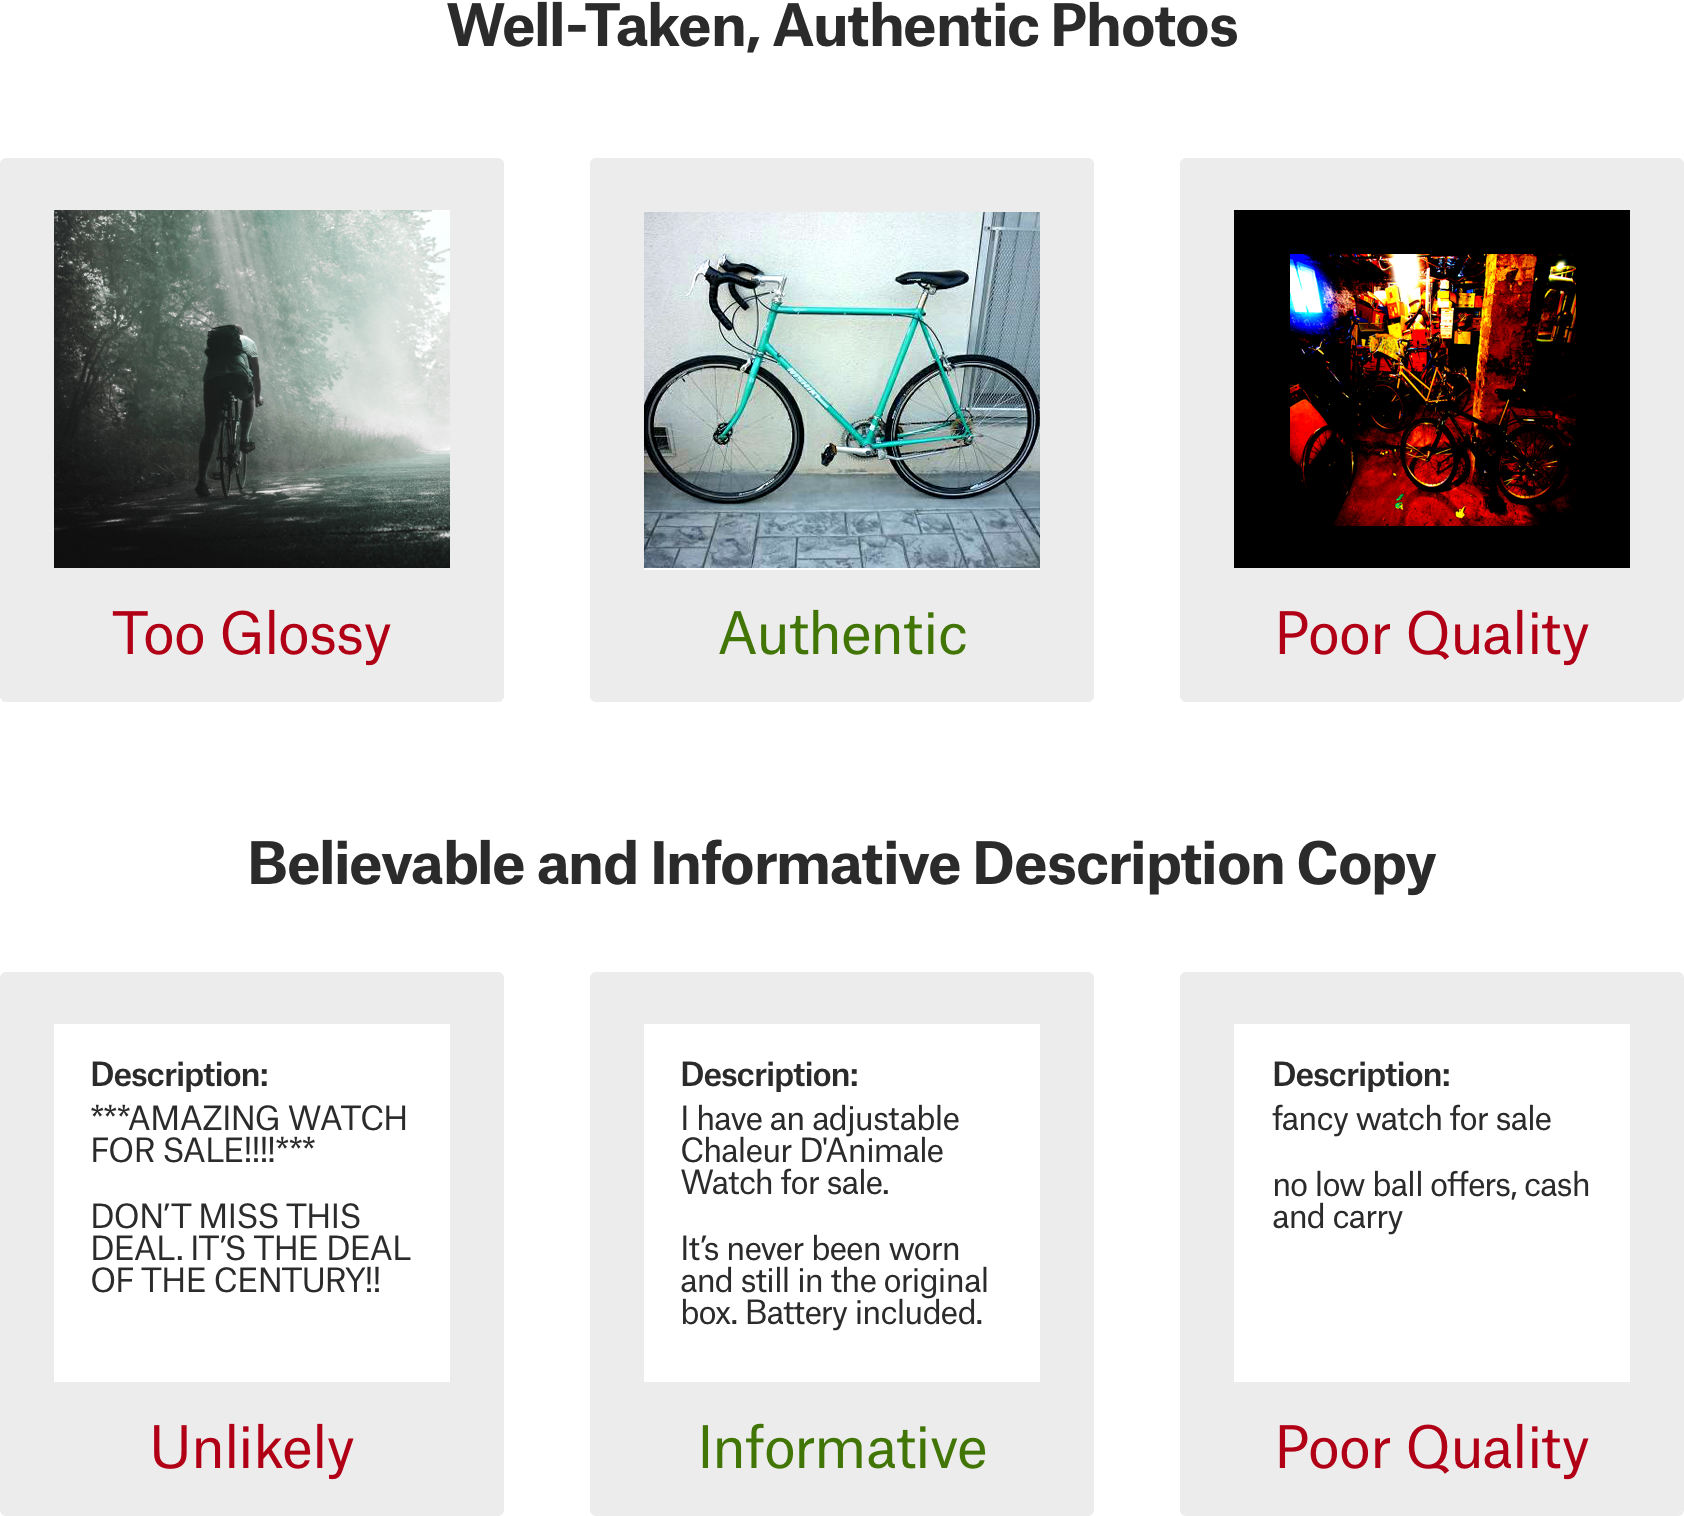
\includegraphics{./statement.png}
\caption{alt text}
\end{figure}

And, even with an optimized product listing, demand for a product may
simply not exist--frustrating sellers who may have over-invested in
marketing. Avito, Russia's largest classified advertisements website, is
deeply familiar with this problem. Sellers on their platform sometimes
feel frustrated with both too little demand (indicating something is
wrong with the product or the product listing) or too much demand
(indicating a hot item with a good description was underpriced). In this
Kaggle competition, Avito is challenging to predict demand for an online
advertisement based on its full description (title, description, images,
etc.), its context (geographically where it was posted, similar ads
already posted) and historical demand for similar ads in similar
contexts. With this information, Avito can inform sellers on how to best
optimize their listing and provide some indication of how much interest
they should realistically expect to receive.

I want to take a subset of their data to test and verify how prediction
by details help a user to get best price of their product.

I will be treating this problem as Regression one. As the value can be
in {[}0,1{]} both inclusive, as we can never be sure 100\% of ad demand.

    \subsubsection{Metrics}\label{metrics}

    Metrics are used to evaluate how our algorithms are working. As per the
Kaggle challenge, I will be using the following metric:

    \[ RMSE = {\sqrt{ \sum_{i=1}^n (y - y_i ̂  )^2 \over n } } \]

    Where

\[ predicted Value => y_i ̂  \]

\[ original Value => y \]

    \subsection{II. Analysis}\label{ii.-analysis}

    \subsubsection{Data Exploration}\label{data-exploration}

    \begin{Verbatim}[commandchars=\\\{\}]
{\color{incolor}In [{\color{incolor}1}]:} \PY{k+kn}{import} \PY{n+nn}{numpy} \PY{k}{as} \PY{n+nn}{np}
        \PY{k+kn}{import} \PY{n+nn}{pandas} \PY{k}{as} \PY{n+nn}{pd}
        
        \PY{k+kn}{import} \PY{n+nn}{seaborn} \PY{k}{as} \PY{n+nn}{sns}
        \PY{k+kn}{import} \PY{n+nn}{matplotlib}\PY{n+nn}{.}\PY{n+nn}{pyplot} \PY{k}{as} \PY{n+nn}{plt}
\end{Verbatim}


    Dataset is available under challenge:
https://www.kaggle.com/c/avito-demand-prediction/data

\begin{itemize}
\tightlist
\item
  train.csv - Train data

  \begin{itemize}
  \tightlist
  \item
    item\_id - Ad id
  \item
    user\_id - User id
  \item
    region - Ad region
  \item
    city - Ad city
  \item
    parent\_category\_name - Top level ad category as classified by
    Avito's ad model
  \item
    category\_name - Fine grain ad category as classified by Avito's ad
    model
  \item
    param\_1 - Optional parameter from Avito's ad model
  \item
    param\_2 - Optional parameter from Avito's ad model
  \item
    param\_3 - Optional parameter from Avito's ad model
  \item
    title - Ad title
  \item
    description - Ad description
  \item
    price - Ad price
  \item
    item\_seq\_number - Ad sequential number for user
  \item
    activation\_date- Date ad was placed
  \item
    user\_type - User type
  \item
    image - Id code of image. Ties to a jpg file in train\_jpg. Not
    every ad has an image
  \item
    image\_top\_1 - Avito's classification code for the image
  \item
    deal\_probability - The target variable. This is the likelihood that
    an ad actually sold something. It's not possible to verify every
    transaction with certainty, so this column's value can be any float
    from zero to one
  \end{itemize}
\item
  test.csv - Test data. Same schema as the train data, minus
  deal\_probability
\end{itemize}

    \begin{Verbatim}[commandchars=\\\{\}]
{\color{incolor}In [{\color{incolor}2}]:} \PY{n}{all\PYZus{}train\PYZus{}dataset} \PY{o}{=} \PY{n}{pd}\PY{o}{.}\PY{n}{read\PYZus{}csv}\PY{p}{(}\PY{l+s+s2}{\PYZdq{}}\PY{l+s+s2}{./inputs/train.csv}\PY{l+s+s2}{\PYZdq{}}\PY{p}{)}
        \PY{n}{all\PYZus{}train\PYZus{}dataset}\PY{o}{.}\PY{n}{head}\PY{p}{(}\PY{p}{)}
\end{Verbatim}


\begin{Verbatim}[commandchars=\\\{\}]
{\color{outcolor}Out[{\color{outcolor}2}]:}         item\_id       user\_id                 region              city  \textbackslash{}
        0  b912c3c6a6ad  e00f8ff2eaf9   Свердловская область      Екатеринбург   
        1  2dac0150717d  39aeb48f0017      Самарская область            Самара   
        2  ba83aefab5dc  91e2f88dd6e3     Ростовская область    Ростов-на-Дону   
        3  02996f1dd2ea  bf5cccea572d              Татарстан  Набережные Челны   
        4  7c90be56d2ab  ef50846afc0b  Волгоградская область         Волгоград   
        
          parent\_category\_name               category\_name  \textbackslash{}
        0          Личные вещи  Товары для детей и игрушки   
        1      Для дома и дачи           Мебель и интерьер   
        2  Бытовая электроника               Аудио и видео   
        3          Личные вещи  Товары для детей и игрушки   
        4            Транспорт                  Автомобили   
        
                               param\_1     param\_2 param\_3                  title  \textbackslash{}
        0    Постельные принадлежности         NaN     NaN  Кокоби(кокон для сна)   
        1                       Другое         NaN     NaN      Стойка для Одежды   
        2  Видео, DVD и Blu-ray плееры         NaN     NaN         Philips bluray   
        3         Автомобильные кресла         NaN     NaN             Автокресло   
        4                   С пробегом  ВАЗ (LADA)    2110         ВАЗ 2110, 2003   
        
                                                 description    price  \textbackslash{}
        0  Кокон для сна малыша,пользовались меньше месяц{\ldots}    400.0   
        1          Стойка для одежды, под вешалки. С бутика.   3000.0   
        2  В хорошем состоянии, домашний кинотеатр с blu {\ldots}   4000.0   
        3                             Продам кресло от0-25кг   2200.0   
        4                           Все вопросы по телефону.  40000.0   
        
           item\_seq\_number activation\_date user\_type  \textbackslash{}
        0                2      2017-03-28   Private   
        1               19      2017-03-26   Private   
        2                9      2017-03-20   Private   
        3              286      2017-03-25   Company   
        4                3      2017-03-16   Private   
        
                                                       image  image\_top\_1  \textbackslash{}
        0  d10c7e016e03247a3bf2d13348fe959fe6f436c1caf64c{\ldots}       1008.0   
        1  79c9392cc51a9c81c6eb91eceb8e552171db39d7142700{\ldots}        692.0   
        2  b7f250ee3f39e1fedd77c141f273703f4a9be59db4b48a{\ldots}       3032.0   
        3  e6ef97e0725637ea84e3d203e82dadb43ed3cc0a1c8413{\ldots}        796.0   
        4  54a687a3a0fc1d68aed99bdaaf551c5c70b761b16fd0a2{\ldots}       2264.0   
        
           deal\_probability  
        0           0.12789  
        1           0.00000  
        2           0.43177  
        3           0.80323  
        4           0.20797  
\end{Verbatim}
            
    \begin{Verbatim}[commandchars=\\\{\}]
{\color{incolor}In [{\color{incolor}3}]:} \PY{n}{all\PYZus{}test\PYZus{}dataset} \PY{o}{=} \PY{n}{pd}\PY{o}{.}\PY{n}{read\PYZus{}csv}\PY{p}{(}\PY{l+s+s2}{\PYZdq{}}\PY{l+s+s2}{./inputs/test.csv}\PY{l+s+s2}{\PYZdq{}}\PY{p}{)}
        \PY{n}{all\PYZus{}test\PYZus{}dataset}\PY{o}{.}\PY{n}{head}\PY{p}{(}\PY{p}{)}
\end{Verbatim}


\begin{Verbatim}[commandchars=\\\{\}]
{\color{outcolor}Out[{\color{outcolor}3}]:}         item\_id       user\_id                 region         city  \textbackslash{}
        0  6544e41a8817  dbe73ad6e4b5  Волгоградская область    Волгоград   
        1  65b9484d670f  2e11806abe57   Свердловская область  Нижняя Тура   
        2  8bab230b2ecd  0b850bbebb10  Новосибирская область       Бердск   
        3  8e348601fefc  5f1d5c3ce0da    Саратовская область      Саратов   
        4  8bd2fe400b89  23e2d97bfc7f   Оренбургская область      Бузулук   
        
          parent\_category\_name               category\_name                 param\_1  \textbackslash{}
        0          Личные вещи      Детская одежда и обувь           Для мальчиков   
        1        Хобби и отдых                  Велосипеды                Дорожные   
        2  Бытовая электроника               Аудио и видео  Телевизоры и проекторы   
        3      Для дома и дачи             Бытовая техника               Для кухни   
        4          Личные вещи  Товары для детей и игрушки         Детские коляски   
        
           param\_2 param\_3              title  \textbackslash{}
        0    Обувь      25    Отдам бесплатно   
        1      NaN     NaN   Продам велосипед   
        2      NaN     NaN                BBK   
        3  Вытяжки     NaN  Вытяжка Jetair 60   
        4      NaN     NaN  Коляска зима-лето   
        
                                                 description    price  \textbackslash{}
        0                                       На ангарском      NaN   
        1  Продам велосипед KAMA  F200,в нормальном состо{\ldots}   3000.0   
        2  Продам новый телевизор BBK  32 диагональ смарт{\ldots}  15000.0   
        3  Продам новую вытяжку в упаковке,с документами{\ldots}   4500.0   
        4  Продам отличную коляску. б/у 1 год. все вопрос{\ldots}   4900.0   
        
           item\_seq\_number activation\_date user\_type  \textbackslash{}
        0               66      2017-04-18   Private   
        1                4      2017-04-16   Private   
        2               15      2017-04-17   Private   
        3               70      2017-04-17   Private   
        4               15      2017-04-15   Private   
        
                                                       image  image\_top\_1  
        0  a8b57acb5ab304f9c331ac7a074219aed4d349d8aef386{\ldots}       2020.0  
        1                                                NaN          NaN  
        2  8c361112cb049745ef2d1b0ae73594fc5c107286b0c942{\ldots}       2960.0  
        3                                                NaN          NaN  
        4  bc3cf6deef10840fc302e38eb48fa7748aa1e28d534f8f{\ldots}       1002.0  
\end{Verbatim}
            
    \subsubsection{Exploratory
Visualization}\label{exploratory-visualization}

    \paragraph{Abstract Data:}\label{abstract-data}

\begin{itemize}
\tightlist
\item
  Training Data have about 1503424 rows.
\item
  Testing data have 508438.
\item
  I will do split of data in training set and validation set in ratio of
  0.75:0.25.
\item
  Deal\_probability will be the target column.
\end{itemize}

    \begin{Verbatim}[commandchars=\\\{\}]
{\color{incolor}In [{\color{incolor}4}]:} \PY{n}{train\PYZus{}output} \PY{o}{=} \PY{n}{all\PYZus{}train\PYZus{}dataset}\PY{p}{[}\PY{l+s+s1}{\PYZsq{}}\PY{l+s+s1}{deal\PYZus{}probability}\PY{l+s+s1}{\PYZsq{}}\PY{p}{]}\PY{o}{.}\PY{n}{astype}\PY{p}{(}\PY{l+s+s1}{\PYZsq{}}\PY{l+s+s1}{float32}\PY{l+s+s1}{\PYZsq{}}\PY{p}{)}
        \PY{n}{train\PYZus{}input} \PY{o}{=} \PY{n}{all\PYZus{}train\PYZus{}dataset}\PY{o}{.}\PY{n}{drop}\PY{p}{(}\PY{p}{[}\PY{l+s+s1}{\PYZsq{}}\PY{l+s+s1}{deal\PYZus{}probability}\PY{l+s+s1}{\PYZsq{}}\PY{p}{]}\PY{p}{,} \PY{n}{axis}\PY{o}{=}\PY{l+m+mi}{1}\PY{p}{)}
        \PY{c+c1}{\PYZsh{} del all\PYZus{}train\PYZus{}dataset[\PYZsq{}deal\PYZus{}probability\PYZsq{}] \PYZsh{}\PYZsh{}\PYZsh{}\PYZsh{}\PYZsh{}\PYZsh{} can be used}
        \PY{n}{test\PYZus{}input} \PY{o}{=} \PY{n}{all\PYZus{}test\PYZus{}dataset}\PY{o}{.}\PY{n}{copy}\PY{p}{(}\PY{p}{)}
\end{Verbatim}


    \begin{Verbatim}[commandchars=\\\{\}]
{\color{incolor}In [{\color{incolor}5}]:} \PY{n}{plt}\PY{o}{.}\PY{n}{figure}\PY{p}{(}\PY{n}{figsize}\PY{o}{=}\PY{p}{(}\PY{l+m+mi}{20}\PY{p}{,} \PY{l+m+mi}{8}\PY{p}{)}\PY{p}{)}
        \PY{n}{all\PYZus{}train\PYZus{}dataset}\PY{o}{.}\PY{n}{region}\PY{o}{.}\PY{n}{value\PYZus{}counts}\PY{p}{(}\PY{n}{dropna}\PY{o}{=}\PY{k+kc}{False}\PY{p}{)}\PY{o}{.}\PY{n}{plot}\PY{p}{(}\PY{n}{kind}\PY{o}{=}\PY{l+s+s1}{\PYZsq{}}\PY{l+s+s1}{bar}\PY{l+s+s1}{\PYZsq{}}\PY{p}{,} \PY{n}{rot}\PY{o}{=}\PY{l+m+mi}{0}\PY{p}{)}
        \PY{n}{plt}\PY{o}{.}\PY{n}{xlabel}\PY{p}{(}\PY{l+s+s1}{\PYZsq{}}\PY{l+s+s1}{Region}\PY{l+s+s1}{\PYZsq{}}\PY{p}{)}
        \PY{n}{plt}\PY{o}{.}\PY{n}{xticks}\PY{p}{(}\PY{n}{rotation}\PY{o}{=}\PY{l+m+mi}{90}\PY{p}{)}
        \PY{n}{sns}\PY{o}{.}\PY{n}{despine}\PY{p}{(}\PY{p}{)}
\end{Verbatim}


    \begin{center}
    \adjustimage{max size={0.9\linewidth}{0.9\paperheight}}{output_20_0.png}
    \end{center}
    { \hspace*{\fill} \\}
    
    \begin{Verbatim}[commandchars=\\\{\}]
{\color{incolor}In [{\color{incolor}6}]:} \PY{n}{plt}\PY{o}{.}\PY{n}{figure}\PY{p}{(}\PY{n}{figsize}\PY{o}{=}\PY{p}{(}\PY{l+m+mi}{20}\PY{p}{,} \PY{l+m+mi}{8}\PY{p}{)}\PY{p}{)}
        \PY{n}{all\PYZus{}train\PYZus{}dataset}\PY{o}{.}\PY{n}{category\PYZus{}name}\PY{o}{.}\PY{n}{value\PYZus{}counts}\PY{p}{(}\PY{n}{dropna}\PY{o}{=}\PY{k+kc}{False}\PY{p}{)}\PY{o}{.}\PY{n}{plot}\PY{p}{(}\PY{n}{kind}\PY{o}{=}\PY{l+s+s1}{\PYZsq{}}\PY{l+s+s1}{bar}\PY{l+s+s1}{\PYZsq{}}\PY{p}{,} \PY{n}{rot}\PY{o}{=}\PY{l+m+mi}{0}\PY{p}{)}
        \PY{n}{plt}\PY{o}{.}\PY{n}{xlabel}\PY{p}{(}\PY{l+s+s1}{\PYZsq{}}\PY{l+s+s1}{Category Name}\PY{l+s+s1}{\PYZsq{}}\PY{p}{)}
        \PY{n}{plt}\PY{o}{.}\PY{n}{xticks}\PY{p}{(}\PY{n}{rotation}\PY{o}{=}\PY{l+m+mi}{90}\PY{p}{)}
        \PY{n}{sns}\PY{o}{.}\PY{n}{despine}\PY{p}{(}\PY{p}{)}
\end{Verbatim}


    \begin{center}
    \adjustimage{max size={0.9\linewidth}{0.9\paperheight}}{output_21_0.png}
    \end{center}
    { \hspace*{\fill} \\}
    
    \begin{Verbatim}[commandchars=\\\{\}]
{\color{incolor}In [{\color{incolor}7}]:} \PY{n}{plt}\PY{o}{.}\PY{n}{figure}\PY{p}{(}\PY{n}{figsize}\PY{o}{=}\PY{p}{(}\PY{l+m+mi}{20}\PY{p}{,} \PY{l+m+mi}{8}\PY{p}{)}\PY{p}{)}
        \PY{n}{all\PYZus{}train\PYZus{}dataset}\PY{o}{.}\PY{n}{parent\PYZus{}category\PYZus{}name}\PY{o}{.}\PY{n}{value\PYZus{}counts}\PY{p}{(}\PY{n}{dropna}\PY{o}{=}\PY{k+kc}{False}\PY{p}{)}\PY{o}{.}\PY{n}{plot}\PY{p}{(}\PY{n}{kind}\PY{o}{=}\PY{l+s+s1}{\PYZsq{}}\PY{l+s+s1}{bar}\PY{l+s+s1}{\PYZsq{}}\PY{p}{,} \PY{n}{rot}\PY{o}{=}\PY{l+m+mi}{0}\PY{p}{)}
        \PY{n}{plt}\PY{o}{.}\PY{n}{xlabel}\PY{p}{(}\PY{l+s+s1}{\PYZsq{}}\PY{l+s+s1}{Parent Category Name}\PY{l+s+s1}{\PYZsq{}}\PY{p}{)}
        \PY{n}{plt}\PY{o}{.}\PY{n}{xticks}\PY{p}{(}\PY{n}{rotation}\PY{o}{=}\PY{l+m+mi}{90}\PY{p}{)}
        \PY{n}{sns}\PY{o}{.}\PY{n}{despine}\PY{p}{(}\PY{p}{)}
        \PY{c+c1}{\PYZsh{} plt.figure(figsize=(20, 8))}
        \PY{c+c1}{\PYZsh{} all\PYZus{}train\PYZus{}dataset.city.value\PYZus{}counts(dropna=False).plot(kind=\PYZsq{}bar\PYZsq{}, rot=0)}
        \PY{c+c1}{\PYZsh{} plt.xlabel(\PYZsq{}city\PYZsq{})}
        \PY{c+c1}{\PYZsh{} plt.xticks(rotation=90)}
        \PY{c+c1}{\PYZsh{} sns.despine()}
        
        \PY{c+c1}{\PYZsh{} plt.figure(figsize=(20, 8))}
        \PY{c+c1}{\PYZsh{} all\PYZus{}train\PYZus{}dataset.price.value\PYZus{}counts(dropna=False).plot(kind=\PYZsq{}bar\PYZsq{}, rot=0)}
        \PY{c+c1}{\PYZsh{} plt.xlabel(\PYZsq{}city\PYZsq{})}
        \PY{c+c1}{\PYZsh{} plt.xticks(rotation=90)}
        \PY{c+c1}{\PYZsh{} sns.despine()}
\end{Verbatim}


    \begin{center}
    \adjustimage{max size={0.9\linewidth}{0.9\paperheight}}{output_22_0.png}
    \end{center}
    { \hspace*{\fill} \\}
    
    \subsubsection{Algorithms and
Techniques}\label{algorithms-and-techniques}

    As this is a supervised learning problem with a regression solution with
range {[}0,1{]}; I want to use different ensemble methods with tuning of
hyper-parameters for the best model later for improvements. I tried with
following algorithms: - XGBRegressor - GradientBoostingRegressor -
AdaBoostRegressor - CatBoostRegressor

    \subsubsection{Benchmark}\label{benchmark}

    As this is like a recommended system, I used Decision tree as with
GridSearchCV as hyperparameter tuning to save its best model.

    \subsection{III. Methodology}\label{iii.-methodology}

    \subsubsection{Data Preprocessing}\label{data-preprocessing}

    \begin{itemize}
\tightlist
\item
  Data preprocessing/cleaning

  \begin{itemize}
  \tightlist
  \item
    Text data will be one-hot encoded for the required text columns
    (except for item\_id, user\_id, title, description).
  \item
    As I will be working with csv data, Image related columns converted
    to bool type.
  \item
    For Outliers detection, I will be using Interquartile range process.
  \item
    filled the missing values with some constant.
  \item
    Split data into training \& validation set
  \end{itemize}
\end{itemize}

    \subsubsection{Implementation}\label{implementation}

    \begin{itemize}
\tightlist
\item
  Evaluate Algorithm

  \begin{itemize}
  \tightlist
  \item
    Build Models (try in between AdaBoost, GradientBoost, Lightgbm,
    Xgboost, Catboost)
  \item
    Select best model
  \item
    Make predictions on validation set
  \end{itemize}
\end{itemize}

    \subsubsection{Refinement}\label{refinement}

    \begin{itemize}
\tightlist
\item
  Model tuning to improve results

  \begin{itemize}
  \tightlist
  \item
    Select best model with tuning hyper-parameters. First I will choose
    a range of parameters in some step increments \& also some
    randomized values for covering large parameter space also.
  \end{itemize}
\end{itemize}

    \subsection{IV. Results}\label{iv.-results}

    \subsubsection{Model Evaluation and
Validation}\label{model-evaluation-and-validation}

    If the trained model is giving me accuracy upto what I want or similar
to kaggle competition, I will be satisfied. I will create custom
ensemble model, if required for fallback if nothing work to my
expectations.

    \subsubsection{Justification}\label{justification}

    \subsection{V. Conclusion}\label{v.-conclusion}

    Submission @Kaggle of csv file.

\begin{figure}
\centering
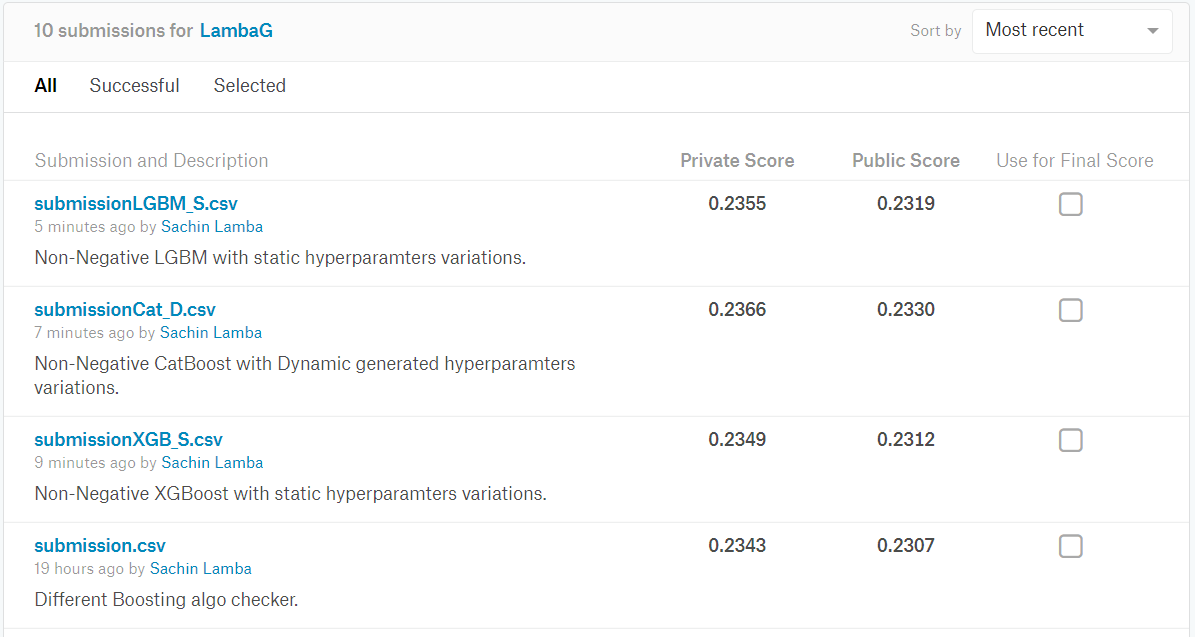
\includegraphics{./submissions.png}
\caption{alt text}
\end{figure}

    \subsubsection{Free-Form Visualization}\label{free-form-visualization}

    \subsubsection{Reflection}\label{reflection}

    \subsubsection{Improvement}\label{improvement}

    Their can be various improvements try: - One can be to use fasttext for
text conversion to word vector. I need to read about more about NLP for
that so that those text columns can be utilized by boosting algorithms.
- Use Computer vision to have images tell about product sentiments. It
can help more in deducing the probability of buyer interest to some
extent.


    % Add a bibliography block to the postdoc
    
    
    
    \end{document}
